\documentclass{article}
\usepackage{fullpage}
\usepackage{indentfirst}
\usepackage{amsmath}
\usepackage{amsfonts}
\usepackage{array}
\usepackage{tipa}
\usepackage{tikz}
\usepackage{tikz-qtree}
\usepackage[backend=bibtex8]{biblatex}
\addbibresource{references.bib}
\usetikzlibrary{matrix, arrows, automata}
\usepackage{gb4e}
\noautomath
\newcommand{\Y}{$\checkmark$}
\newcommand{\N}{\ding{55}}
\newcommand{\R}{$\Rightarrow$}
\title{
	Sandhi with Chao Letters and MC Categories \\
	\large (Using Rules and FSTs)
	}
\author{Chris Oakden}
\begin{document}
\maketitle
This is the basic format we're going to work with here:
\begin{itemize}
	\item The entire inventory of lexical tones
	\item A rule (or rules) using tone letters, and then using traditional categories
	\item Consider the inverse of the rule as part of the logical possibilities (in discussion?)
	\item FSTs (also using letters and then traditional categories?)
\end{itemize}
In a separate section at the end, discuss generalizations
\section{Rizhao (Mandarin)}
Rizhao is a Mandarin dialect spoken in Shandong province.\cite{Wuandliu2010}
\begin{exe}
\ex Tonal Inventory \\
\begin{tabular}[t]{|ll|}
\hline
Category & Chao Letters \\
\textit{yinping} & 214 \\
\textit{yangping} & 53 \\
\textit{shang} & 55 \\
\textit{qu} & 31 \\
\hline
\end{tabular}
\end{exe}
Attested disyllabic sandhi patterns are below in Chao tone letters and in MC categories. Note that many sandhi tones do not have a MC lexical equivalent, so they are designated with prime or double-prime where appropriate.
\begin{exe}
\ex
\begin{tabular}[t]{ll}
Chao Letters & MC Categories \\
\hline
214 $\rightarrow$ 24 / \underline{\hspace{1em}} 214, 31 & \textit{yinp} $\rightarrow$ \textit{yinp}$'$ / \underline{\hspace{1em}} \textit{yinp}, \textit{qu} \\
214 $\rightarrow$ 213 / \underline{\hspace{1em}} 53, 55 & \textit{yinp} $\rightarrow$ \textit{yinp}$''$ / \underline{\hspace{1em}} \textit{yangp}, \textit{shang} \\
53 $\rightarrow$ 54 / \underline{\hspace{1em}} 53 & \textit{yangp} $\rightarrow$ \textit{yangp}$'$ / \underline{\hspace{1em}} \textit{yangp} \\
53 $\rightarrow$ 24 / \underline{\hspace{1em}} 31 & \textit{yangp} $\rightarrow$ \textit{yangp}$''$ / \underline{\hspace{1em}} \textit{qu} \\
55 $\rightarrow$ 53 / \underline{\hspace{1em}} 55 & \textit{shang} $\rightarrow$ \textit{shang}$'$ / \underline{\hspace{1em}} \textit{shang} \\
31 $\rightarrow$ 24 / \underline{\hspace{1em}} 31 & \textit{qu} $\rightarrow$ \textit{qu}$'$ / \underline{\hspace{1em}} \textit{qu} \\ \\
\end{tabular}
\end{exe}
The `elsewhere' case for \textit{yinping} is accounted for. Surprisingly, its citation form never occurs in initial position in a disyllabic sandhi environment. The other `elsewhere' cases are outlined below:
\begin{exe}
\ex 
\begin{xlist}
\ex \textit{yangping} \\
53 $\rightarrow$ 53 / \underline{\hspace{1em}} 214, 55
\ex \textit{shang} \\
55 $\rightarrow$ 55 / \underline{\hspace{1em}} 214, 53, 31
\ex \textit{qu} \\
31 $\rightarrow$ 31 / \underline{\hspace{1em}} 214, 53, 55
\end{xlist}
\end{exe}
This is a preliminary attempt at constructing an FST for just the 53.T patterns.
\begin{exe}
\ex
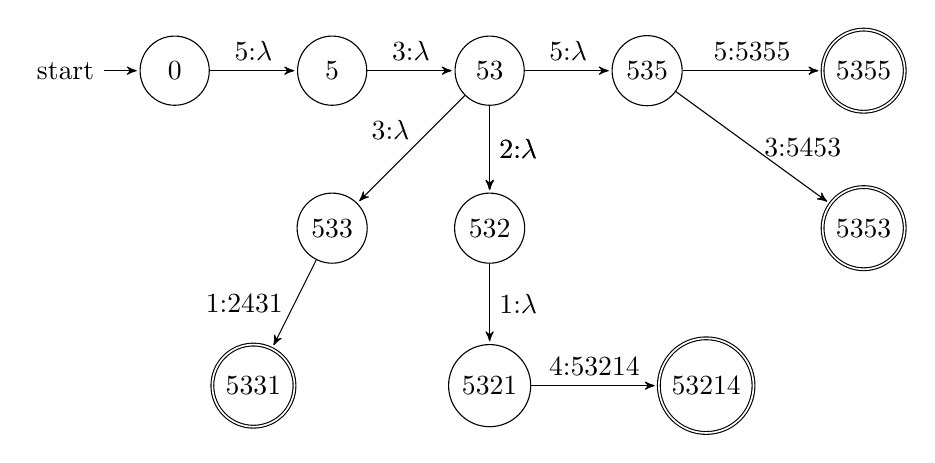
\begin{tikzpicture}[->,>=stealth', shorten >=1pt, auto, node distance = 2cm, baseline = 5]
\node[state, initial](0){0};
\node[state](5)[right of = 0]{5};
\node[state](53)[right of = 5]{53};
\node[state](535)[right of = 53]{535};
\node[state,accepting](5355)[right of = 535, xshift=.75cm]{5355};
\node[state, accepting](5353)[below of = 5355]{5353};
\node[state](533)[below of = 5]{533};
\node[state](532)[below of = 53]{532};
\node[state, accepting](5331)[below of = 533, xshift=-1cm]{5331};
\node[state](5321)[below of = 532]{5321};
\node[state, accepting](53214)[right of = 5321, xshift=.75cm]{53214};
\path (0) edge node {5:$\lambda$} (5);
\path (5) edge node {3:$\lambda$} (53);
\path (53) edge node {5:$\lambda$} (535);
\path (535) edge node {5:5355} (5355);
\path (53) edge node [above, text width = 1cm, align=left] {3:$\lambda$} (533);
\path (533) edge node [left, text width = 1cm, align=left] {1:2431} (5331);
\path (53) edge node [right, align=right] {2:$\lambda$} (532);
\path (53) edge node [right, align=right] {2:$\lambda$} (532);
\path (532) edge node [right, align=right] {1:$\lambda$} (5321);
\path (5321) edge node {4:53214} (53214);
\path (535) edge node [right, text width = 1cm, align = right] {3:5453} (5353);
\end{tikzpicture}
\end{exe}
\section{Hefei (Mandarin)}
Hefei is a Mandarin dialect spoken in Anhui province.\cite{Kong2008}
\begin{exe}
\ex Tonal Inventory \\
\begin{tabular}[t]{|ll|}
\hline
Category & Chao Letters \\
\textit{yinping} & 21 \\
\textit{yangping} & 55 \\
\textit{shang} & 24 \\
\textit{qu} &  53 \\
\textit{ru} & 5q \\
\hline
\end{tabular}
\end{exe}
Attested disyllabic sandhi patterns are below in Chao tone letters and in MC categories.
\begin{exe}
\ex
\begin{tabular}[t]{ll}
Chao Letters & MC Categories \\
\hline
21 $\rightarrow$ 24 / \underline{\hspace{1em}} 21, 53 & \textit{yinp} $\rightarrow$ \textit{shang} / \underline{\hspace{1em}} \textit{yinp, qu} \\ 
5q $\rightarrow$ 2q / \underline{\hspace{1em}} 55, 24, 5q & \textit{ru} $\rightarrow$ \textit{ru}$'$ / \underline{\hspace{1em}} \textit{yangp, shang, ru} \\ 
\end{tabular}
\end{exe}
Elsewhere cases are outlined below for each tone which undergoes sandhi.
\begin{exe}
\ex 
\begin{xlist}
\ex \textit{yinping} \\
21 $\rightarrow$ 21 / \underline{\hspace{1em}} 55, 24, 5q
\ex \textit{ru} \\
5q $\rightarrow$ 5q / \underline{\hspace{1em}} 21, 53
\end{xlist}
\end{exe}
\section{Yinchuan (Mandarin)}
Yinchuan is a Mandarin dialect spoken in Ningxia province.\cite{Zhang1984} Strangely, the author splits \textit{shang} into two categories based on sandhi: \textit{shangjia} and \textit{shangyi}. Their pronunciation in isolation is the same, but differs in sandhi contexts.
\begin{exe}
\ex Tonal Inventory \\
\begin{tabular}[t]{|ll|}
\hline
Category & Chao Letters \\
\textit{ping} & 44 \\
\textit{shangjia} & 53 \\
\textit{shangyi} & 53 \\
\textit{qu} &  14 \\
\hline
\end{tabular}
\end{exe}
One sandhi alternation is reported.
\begin{exe}
\ex
\begin{tabular}[t]{ll}
Chao Letters & MC Categories \\
\hline
53 $\rightarrow$ 35 / \underline{\hspace{1em}} 14 & \textit{shangyi} $\rightarrow$ \textit{shangyi}$'$ / \underline{\hspace{1em}} \textit{qu} \\ 
\end{tabular}
\end{exe}
The elsewhere cases for \textit{shangyi} include all other environments, including at a word boundary.
\begin{exe}
\ex 
\begin{xlist}
\ex \textit{shangyi} \\
53 $\rightarrow$ 53 / \underline{\hspace{1em}} 44, 53, \#
\end{xlist}
\end{exe}
\section{Gao'an Laowu Zhoujia (Gan)}
Gao'an is a Gan dialect spoken in Jiangxi province.\cite{Yan1981}
\begin{exe}
\ex Tonal Inventory \\
\begin{tabular}[t]{|ll|}
\hline
Category & Chao Letters \\
\textit{yinping} & 55 \\
\textit{yangping} & 24 \\
\textit{shang} & 42 \\
\textit{yinqu} &  33 \\
\textit{yangqu} & 11 \\
\textit{yinru} & 3q \\
\textit{yangru} & 1q \\
\hline
\end{tabular}
\end{exe}
One tone sandhi alternation is reported for Gao'an:
\begin{exe}
\ex
\begin{tabular}[t]{ll}
Chao Letters & MC Categories \\
\hline
55 $\rightarrow$ 53 / \underline{\hspace{1em}} 33, 31, 3q, 1q & \textit{yinp} $\rightarrow$ \textit{yinp}$'$ / \underline{\hspace{1em}} \textit{yinqu, yangqu, yinru, yangru} \\ 
\end{tabular}
\end{exe}
Elsewhere cases are outlined below for \textit{yinping}:
\begin{exe}
\ex 
\begin{xlist}
\ex \textit{yinping} \\
55 $\rightarrow$ 55 / \underline{\hspace{1em}} 55, 42, 24
\end{xlist}
\end{exe}
\section{Zhangping (Min)}
Zhangping is a Min dialect spoken in Fujian province.\cite{Zhang1982, chen2000}
\begin{exe}
\ex Tonal Inventory \\
\begin{tabular}[t]{|ll|}
\hline
Category & Chao Letters \\
\textit{yinping} & 24 \\
\textit{yangping} & 11 \\
\textit{yinshang} & 31 \\
\textit{yinqu} &  21 \\
\textit{yangqu} & 53 \\
\textit{yinru} & 5q \\
\textit{yangru} & 53q \\
\hline
\end{tabular}
\end{exe}
Tone sandhi in the dialect is marked by widespread neutralization.
\begin{exe}
\ex
\begin{tabular}[t]{l}
Chao Letters \\
\hline
24, 11, 21, 5q $\rightarrow$ 33 / \underline{\hspace{1em}} 24, 11, 5q, 53, 53q \\ 
24, 11, 21, 5q $\rightarrow$ 55 / \underline{\hspace{1em}} 31, 21 \\
31, 53, 53q $\rightarrow$ 21 / \underline{\hspace{1em}} 24, 11, 5q, 53, 53q \\  
\end{tabular}
\ex
\begin{tabular}[t]{l}
MC Categories \\
\hline
\textit{yinp, yangp, yinqu, yinru} $\rightarrow$ 33 / \underline{\hspace{1em}} \textit{yinp, yangp, yinru, yangqu, yangru} \\
\textit{yinp, yangp, yinqu, yinru} $\rightarrow$ 55 / \underline{\hspace{1em}} \textit{yinshang, yinqu} \\
\textit{yinshang, yangqu, yangru} $\rightarrow$ 21 / \underline{\hspace{1em}} \textit{yinp, yangp, yinru, yangqu, yangru} \\
\end{tabular}
\end{exe}
All environments for 24, 11, 21, and 5q are accounted for. Elsewhere cases for 31, 53, and 5q include:
\begin{exe}
\ex 
\begin{xlist}
\ex \textit{yinshang} \\
31 $\rightarrow$ 31 / \underline{\hspace{1em}} 31, 21 \\
\ex \textit{yangqu} \\
53 $\rightarrow$ 53 / \underline{\hspace{1em}} 31, 21 \\
\ex \textit{yangqu} \\
53q $\rightarrow$ 53q / \underline{\hspace{1em}} 31, 21 \\
\end{xlist}
\end{exe}
\section{Pingyao (Jin)}
Pingyao is a Jin dialect spoken in Shanxi province \cite{Hou1980, chen2000}. Note that \textit{yinping} and \textit{yangping} have the same citation form (but they are differentiated in sandhi environments).
\begin{exe}
\ex Tonal Inventory \\
\begin{tabular}[t]{|ll|}
\hline
Category & Chao Letters \\
\textit{yinping} & 13 \\
\textit{yangping} & 13 \\
\textit{shang} & 53 \\
\textit{qu} & 35 \\
\textit{yinru} & 23q \\
\textit{yangru} & 54q \\
\hline
\end{tabular}
\end{exe}
Pingyao tone sandhi is complex and shows evidence of structure sensitivity. I will focus on \textit{yangping} patterns to simplify. Note that this includes some context free patterns. 
\begin{exe}
\ex
\begin{tabular}[t]{ll}
Chao Letters & MC Categories \\
\hline
13 $\rightarrow$ 31 / \underline{\hspace{1em}} 35 & \textit{yangp} $\rightarrow$ \textit{yangp}$'$ / \underline{\hspace{1em}} \textit{qu} \\ 
13.53 $\rightarrow$ 35513 & \textit{yangp.shang} $\rightarrow$ \textit{yangp}$'$.\textit{shang}$'$ \\ 
13.54q $\rightarrow$ 35513q & \textit{yangp.yangr} $\rightarrow$ \textit{yangp}$'$.\textit{yangr}$'$ \\ 
\end{tabular}
\end{exe}
\textit{Yangping} does not change in other environments, including:
\begin{exe}
\ex 
\begin{xlist}
\ex \textit{yangping} \\
13 $\rightarrow$ 13 / \underline{\hspace{1em}} 13, 23q \\
\end{xlist}
\end{exe}
\section{Yudu (Hakka)}
Yudu is a Hakka dialect spoken in Shanxi province \cite{Xie1992, chen2000}.
\begin{exe}
\ex Tonal Inventory \\
\begin{tabular}[t]{|ll|}
\hline
Category & Chao Letters \\
\textit{yinping} & 31 \\
\textit{yangping} & 44 \\
\textit{shang} & 35 \\
\textit{yinqu} & 22 \\
\textit{yangqu} & 42 \\
\textit{ru} & 5q \\
\hline
\end{tabular}
\end{exe}
I will simplify the \textit{yinqu} patterns in describing sandhi, describing only the rule in which it surfaces as 44 at word edges. In other positions, its distribution is structure sensitive, with a subset of its morphemes surfacing as \textit{rusheng} in certain contexts. 
\begin{exe}
\ex
\begin{tabular}[t]{ll}
Chao Letters & MC Categories \\
\hline
44 $\rightarrow$ 42 / \underline{\hspace{1em}} 44 & \textit{yangp} $\rightarrow$ \textit{yangp}$'$ / \underline{\hspace{1em}} \textit{yangp} \\ 
35 $\rightarrow$ 31 / \underline{\hspace{1em}} T & \textit{shang} $\rightarrow$ \textit{shang}$'$ / \underline{\hspace{1em}} T \\ 
5q $\rightarrow$ 42q / \underline{\hspace{1em}} T & \textit{ru} $\rightarrow$ \textit{ru}$'$ / \underline{\hspace{1em}} T \\ 
22 $\rightarrow$ 44 / T \underline{\hspace{1em}} & \textit{yinqu} $\rightarrow$ \textit{yinqu}$'$ / T \underline{\hspace{1em}} \\ 
\end{tabular}
\end{exe}
Elsewhere cases are provided below (except for \textit{yinqu}):
\begin{exe}
\ex 
\begin{xlist}
\ex \textit{yangping} \\
44 $\rightarrow$ 44 / \underline{\hspace{1em}} 31, 35, 22, 42, 5q
\ex \textit{shang} \\
35 $\rightarrow$ 35 / \underline{\hspace{1em}} \#
\ex \textit{ru} \\
5q $\rightarrow$ 5q / \underline{\hspace{1em}} \#
\end{xlist}
\end{exe}
\section{Changsha (Xiang)}
Changsha is a Xiang dialect spoken in Hunan; experimental studies claim that the language has no level citation tones. \cite{Liandliu2006} 
\begin{exe}
\ex Tonal Inventory \\
\begin{tabular}[t]{|ll|}
\hline
Category & Chao Letters \\
\textit{yinping} & 23 \\
\textit{yangping} & 13 \\
\textit{shang} & 42 \\
\textit{yinqu} & 45 \\
\textit{yangqu} & 42 \\
\textit{ru} & 24q \\
\hline
\end{tabular}
\end{exe}
Three sandhi processes are reported.
\begin{exe}
\ex
\begin{tabular}[t]{ll}
Chao Letters & MC Categories \\
\hline
21 $\rightarrow$ 22 / \underline{\hspace{1em}} T & \textit{yinqu} $\rightarrow$ \textit{yinqu}$'$ / \underline{\hspace{1em}} T \\ 
42 $\rightarrow$ 33 / T \underline{\hspace{1em}} T & \textit{shang} $\rightarrow$ \textit{shang}$'$ / T  \underline{\hspace{1em}} T \\ 
24q $\rightarrow$ 3q / \underline{\hspace{1em}} T & \textit{ru} $\rightarrow$ \textit{ru}$'$ / \underline{\hspace{1em}} T \\ 
\end{tabular}
\end{exe}
Elsewhere cases for these three tones are thus:
\begin{exe}
\ex 
\begin{xlist}
\ex \textit{yinqu} \\
21 $\rightarrow$ 21 / \underline{\hspace{1em}} \#
\ex \textit{shang} \\
42 $\rightarrow$ 42 / \# \underline{\hspace{1em}} \#
\ex \textit{ru} \\
24q $\rightarrow$ 3q / \underline{\hspace{1em}} \#
\end{xlist}
\end{exe}
\section{Wuyi (Wu)}
Wuyi is an Wu dialect spoken in Zhejiang province. \cite{Fu1984}
\begin{exe}
\ex Tonal Inventory \\
\begin{tabular}[t]{|ll|}
\hline
Category & Chao Letters \\
\textit{yinping} & 24 \\
\textit{yangping} & (2)13 \\
\textit{yinshang} & 55 \\
\textit{yangshang} & 13 \\
\textit{yinqu} & 53 \\
\textit{yangqu} & 31 \\
\textit{yinru} & 5q \\
\textit{yangru} & 212q \\
\hline
\end{tabular}
\end{exe}
Tone sandhi in Wuyi, much like Zhangping, is characterized by widespread neutralization on the initial syllable. Some sandhi forms are structurally determined, and in some cases multiple patterns are observed for syllables of the same category. What is presented below is a simplified version of Wuyi tone sandhi.
\begin{exe}
\ex
\begin{tabular}[t]{ll}
Chao Letters & MC Categories \\
\hline
24 $\rightarrow$ 55 / \underline{\hspace{1em}} T & \textit{yinp} $\rightarrow$ \textit{yinp}$'$ / \underline{\hspace{1em}} T \\ 
13 $\rightarrow$ 55 / \underline{\hspace{1em}} T & \textit{yangp} $\rightarrow$ \textit{yangp}$'$ / \underline{\hspace{1em}} T \\ 
53 $\rightarrow$ 55 / \underline{\hspace{1em}} T & \textit{yinqu} $\rightarrow$ \textit{yinqu}$'$ / \underline{\hspace{1em}} T \\ 
31 $\rightarrow$ 11 / \underline{\hspace{1em}} T & \textit{yangqu} $\rightarrow$ \textit{yangqu}$'$ / \underline{\hspace{1em}} T \\ 
55 $\rightarrow$ 11 / \underline{\hspace{1em}} T & \textit{yinshang} $\rightarrow$ \textit{yinshang}$'$ / \underline{\hspace{1em}} T \\ 
13 $\rightarrow$ 11 / \underline{\hspace{1em}} T & \textit{yinp} $\rightarrow$ \textit{yinp}$'$ / \underline{\hspace{1em}} T \\ 
212q $\rightarrow$ 5q / \underline{\hspace{1em}} T & \textit{yangru} $\rightarrow$ \textit{yangru}$'$ / \underline{\hspace{1em}} T \\ 
\end{tabular}
\end{exe}
 Elsewhere cases are irrelevant here; all environments are accounted for, and citation forms appear in non-initial position.
\section{Ningbo (Wu)}
Ningbo is an Wu dialect spoken in Zhejiang province. \cite{Chan1985}
\begin{exe}
\ex Tonal Inventory \\
\begin{tabular}[t]{|ll|}
\hline
Category & Chao Letters \\
\textit{yinping} & 53 \\
\textit{yangping} & 35 \\
\textit{yinshang} & 424 \\
\textit{yangshang} & 313 \\
\textit{yinqu} & 33 \\
\textit{yangqu} & 213 \\
\textit{yinru} & 5q \\
\textit{yangru} & 34q \\
\hline
\end{tabular}
\end{exe}
Tone sandhi in Ningbo is rather complex, and varies based on a variety of factors, including onset voicing in some cases. Below is just an example of disyllabic forms which begin with \textit{yangping}:
\begin{exe}
\ex
\begin{tabular}[t]{ll}
Chao Letters \\
\hline
35T $\rightarrow$ 2244  \\ 
\end{tabular}
\end{exe}
I'm not yet sure how to formalize this spreading rule in terms of an FST.
\section{Discussion}
Restricting ourselves to Chao tone letters, permutations of citation forms in sandhi processes are broadly divisible into two types: right-edge modification and total modification.
\begin{exe}
\ex
\begin{tabular}[t]{ll|ll}
Total Modification & & Right-edge Modification & \\
\hline
\hline
Pattern & Dialect & Pattern & Dialect \\
\hline
53 $\rightarrow$ 24 & Rizhao & 214 $\rightarrow$ 213 & Rizhao \\
31 $\rightarrow$ 24 & Rizhao & 55 $\rightarrow$ 53 & Gao'an \\
24 $\rightarrow$ 33 & Zhangping & 53 $\rightarrow$ 54 & Rizhao \\
24 $\rightarrow$ 11 & Zhangping & 21 $\rightarrow$ 24 & Hefei \\
5q $\rightarrow$ 42q & Yudu & 35 $\rightarrow$ 31 & Yudu \\
22 $\rightarrow$ 44 & Changsha & 44 $\rightarrow$ 42 & Yudu \\
42 $\rightarrow$ 33 & Changsha & 21 $\rightarrow$ 22 & Changsha \\
24q $\rightarrow$ 3q & Changsha & 13 $\rightarrow$ 11 & Wuyi \\
24 $\rightarrow$ 55 & Wuyi & 53 $\rightarrow$ 55 & Wuyi \\
13 $\rightarrow$ 55 & Wuyi & & \\
55 $\rightarrow$ 11 & Wuyi & & \\
\end{tabular}
\end{exe}
With few exceptions (like 21 $\rightarrow$ 24, an analog of the Mandarin 3rd tone sandhi rule, also analyzable as L $\rightarrow$ LH), the right-edge modification patterns can be characterized as either contour simplification or contour formation. In other words: a level tone becomes a contour, or a contour tone becomes level by modifying the right edge of the tone. This type of pattern is pervasive across dialects. \par
Three patterns do not (necessarily) fit into either generalization. Two are ``inversion''-like patterns on contours (or ``contour metathesis" in Chen's terminology): 53 $\rightarrow$ 35 (Yinchuan) and 13 $\rightarrow$ 31 (Pingyao). The pattern 31 $\rightarrow$ 11 (Wuyi) is ostensibly a ``left-modification'' pattern, the only one that emerged from the survey of these dialects. I would like to suggest that all three are cases of total modification. \par
 The first two inversion patterns are cases of contour switching, so, falling-to-rising and rising-to-falling respectively. In the total modification patterns, the same situation obtains, albeit with non-symmetric phonetic values. Examples include 53 $\rightarrow$ 24 and 31 $\rightarrow$ 24 (falling-to-rising) in Rizhao. In fact, all logical possibilities are observed in the total modification alternations: contour to level, level to contour, level to level, and contour to contour. The ``inversion'' patterns fit into this schema. \par
To determine where 31 $\rightarrow$ 11 fits into this pattern, it is worthwhile to consider what \emph{types} of alternations total vs right modification patterns constitute. All the (arguably) syllable-level OCP sandhi patterns are of the right-edge modification type:
\begin{exe}
\ex
\begin{tabular}[t]{ll}
Modification & Environment \\
\hline
214 $\rightarrow$ 213 & \underline{\hspace{1em}} 214 \\
53 $\rightarrow$ 54 & \underline{\hspace{1em}} 53 \\
21 $\rightarrow$ 24 & \underline{\hspace{1em}} 21 \\
44 $\rightarrow$ 42 & \underline{\hspace{1em}} 44 \\
\end{tabular}
\end{exe}
The majority of total modification patterns, by contrast, are cases of extensive neutralization in non-final position or other non-OCP motivated alternations. These are examples like Zhangping and Wuyi, where multiple tonal categories converge on the same phonetic output in these positions. Viewed in isolation, the pattern 31 $\rightarrow$ 11 appears to be a case of left-edge modification; however, when viewed in its context as a Wuyi neutralization pattern (31, 55, 13 \emph{all} map to 11), a total modification is more felicitous. \par
Where does this leave us in terms of possible vs impossible sandhi patterns? One generalization that seems to emerge from the data is: there is no such thing as a ``left-edge modification'' in right-dominant sandhi patterns, at least not for the syllable-level OCP cases. That is to say, the locus of alternation is the immediate environment between the first and second syllable (note that this is also true of Tianjin and Nanjing, not discussed here). There is, then, an interesting asymmetry in the sandhi patterns under our current assumptions. In terms of Chao tone letters, modification of citation tones either targets the entire tone (usually in neutralization contexts, but not always) or it targets the right edge, but never the left edge. Why? \par
To determine whether this is a locality effect, it will be necessary to analyze left-dominant (non-spreading) patterns and look for the inverse: left-modification but no right-modification. But there are more general questions to ponder about what we mean by \emph{locality}, as well. As a string of symbols, why should 55 $\rightarrow$ 35 / \underline{\hspace{1em}} 55 be non-local (or somehow less local) in comparison to 55 $\rightarrow$ 53? It is clear that, as ISL functions, their k-value is the same (in this case k = 4). Additionally, representation in terms of single units (H, L, R, F) obscures any distinction whatsoever:
\begin{exe}
\ex \label{patternX}
\begin{xlist}
	\ex 55 $\rightarrow$ 53 \underline{\hspace{1em}} 55 $\equiv$ H $\rightarrow$ F \underline{\hspace{1em}} H
	\ex 55 $\rightarrow$ 35 \underline{\hspace{1em}} 55 $\equiv$ H $\rightarrow$ R \underline{\hspace{1em}} H
\end{xlist}
\end{exe}
With this in mind, the crucial difference lies not in the available window the function needs to map an input to an output, but rather \emph{where} in the string the two mappings share a discrepancy.  \par
How would other theories or representations account for this discrepancy? Autosegmental theories can account for local \emph{spreading} patterns via the No-Crossing Constraint. The Gao'an pattern 55 $\rightarrow$ 53 / \underline{\hspace{1em}} 33, 31, ... is simply a case of local regressive spreading:
\begin{exe}
\ex
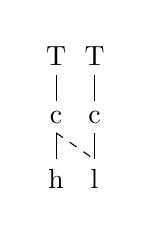
\begin{tikzpicture}[baseline = (m-2-1.base)]
\matrix (m) [matrix of nodes, row sep = 1em]{
T & T \\
c & c \\
h & l \\
};
\draw (m-1-1.south) -- (m-2-1.north);
\draw (m-1-2.south) -- (m-2-2.north);
\draw (m-2-1.south) -- (m-3-1.north);
\draw (m-2-2.south) -- (m-3-2.north);
\draw [dashed] (m-2-1.south) -- (m-3-2.north);
\end{tikzpicture}
\hspace{.75cm} OR \hspace{.75cm}
\begin{tikzpicture}[baseline = (m-2-1.base)]
\matrix (m) [matrix of nodes, row sep = 1em]{
& H & & L & . . . \\
& $\mu$ & $\mu$ & $\mu$ & . . . \\
};
\draw (m-1-2.south) -- (m-2-2.north);
\draw (m-1-2.south) -- (m-2-3.north);
\draw (m-1-4.south) -- (m-2-4.north);
\draw [dashed] (m-1-4.south) -- (m-2-3.north);
\end{tikzpicture}
\end{exe}
In principle, 55 $\rightarrow$ 35 as a case of spreading would be ill-formed.
\begin{exe}
\ex
\begin{tikzpicture}[baseline = (m-2-1.base)]
\matrix (m) [matrix of nodes, row sep = 1em]{
* & H & & L & . . . \\
& $\mu$ & $\mu$ & $\mu$ & . . . \\
};
\draw (m-1-2.south) -- (m-2-2.north);
\draw (m-1-2.south) -- (m-2-3.north);
\draw (m-1-4.south) -- (m-2-4.north);
\draw [dashed] (m-1-4.south) -- (m-2-2.north);
\end{tikzpicture}
\end{exe}
But what about dissimilation, for example Mandarin 3rd tone sandhi (11 $\rightarrow$ 24 / \underline{\hspace{1em}} 11) in which we could argue tonal epenthesis (L $\rightarrow$ L\textbf{H}) obtains? As far as I am aware, ARs have nothing to tell us about why L $\rightarrow$ LH and not *L $\rightarrow$ HL. \par   
In an optimization framework, there are a variety of approaches to privilege right-edge modification over left-edge modification. In my thesis I used a high-ranking \textsc{Anchor} constraint to prefer L $\rightarrow$ LH.
\begin{exe}
\ex
L-\textsc{AnchorT}-[$\sigma$]- Any tonal element at the left edge of a syllable in the input has a correspondent at the left edge of the syllable in the output
\end{exe}
The problem with the above analysis is that, thinking of \textsc{Anchor} constraints in terms of a broad typology, we actually predict its inverse; the existence of L-\textsc{AnchorT}-[$\sigma$] entails another constraint R-\textsc{AnchorT}-[$\sigma$] which under a number of viable total orders would produce the unattested *L $\rightarrow$ HL. Our goal here is not to argue the specifics of an OT analysis of tone, though. What is important to consider is that this approach crucially uses \emph{faithfulness} to derive the attested patterns. In a computational analysis, is there a way to model this? \par
Below are a few miscellaneous points regarding the survey of tone sandhi.
\begin{itemize}
	\item Also take a look at trisyllabic sandhi in Wuyi, because it looks a lot like NJH (ISL)
	\item One of the generalizations you lose from just using tone categories is that there are often phonetically identical sandhi forms which are the same across different categories, so calling an output form xxx$'$ is opaque in a sense. just because citation form of category x is phonetically identical to the sandhi form of category y, do we want to give them the same representation? 
	\item Underlying forms are important! It is often the case that the UR of a citation form only shows up in isolation. so then how do we represent it? 
	\item there is evidence suggesting that underlying representation is arbitrary, especially in neutralization. but then there are others which suggest some sort of local spreading or dissimilation 
	\item phonetic representation explodes the value of k
\end{itemize}
\printbibliography
\end{document}